\documentclass[../../Rapport RayTracer]{subfiles}

\begin{document}


En POV, la définition d'une sphère et d'un plan est exactement la même d'un point de vue syntaxique. 
Afin de gagner en lisibilité et pour factoriser au mieux le code, nous avons donc eu recours à un autre patron de conception: le patron "Template Method".
L'idée de ce pattern est de créer une classe mère abstraite, la classe EtatSpherePlane. Cette classe définit deux types de méthodes:

\begin{itemize}
\item abstraites et qui dépendent donc de la figure
\item concrètes et qui ne dépendent donc pas du type de figure
\end{itemize}

Dans le cas de notre parser, la seule méthode abstraite est celle qui retourne l'objet parsé, la méthode createInstance. C'est normal car on a besoin de savoir si
l'on doit renvoyer une sphère ou un plan.

\begin{figure}[h!]
	\adjustbox{center}{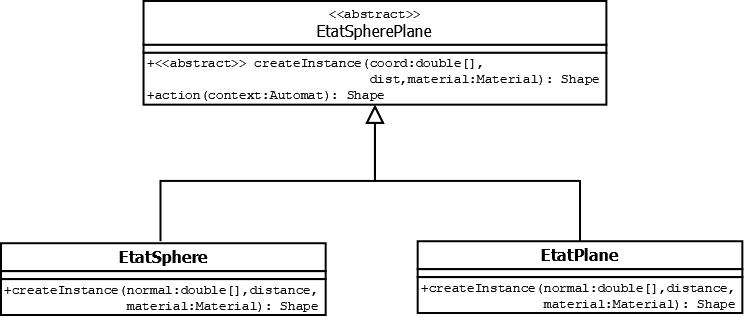
\includegraphics[width=1\textwidth]{diagrammes/pattern_template_method.png}}
	
	\caption{Diagramme du pattern template method appliqué à notre parser}
	\label{diagrammePatternTemplateMethod}
\end{figure}
\FloatBarrier

La méthode qui effectue le parsing, au contraire,  n'a pas besoin de savoir si c'est une sphère ou plan car la syntaxe est exactement la même et donc l'analyse du bloc de figure est aussi la même.

\end{document}